
The non-linear wave equation \eqref{NLW} is the Euler-Lagrange equation arising when one formally considers solutions as critical points of the Lagrangian
	\[
		\cS[\phi] 
			:= \int_{\R^{1 + d}} \frac12 \partial_\alpha \phi \partial^\alpha \phi + \frac{d - 2}{2d} |\phi|^{\frac{2d}{d - 2}} \, dt dx.
	\]
By Noether's principle, the continuous symmetries of the equation lead to conserved quantities. We present the energy-momentum tensor formalism, which is derived from the diffeomorphism-invariance of the Lagrangian. Define the \emph{energy-momentum tensor} by
	\[
		T_{\mu \nu} 
			= \partial_\mu \phi \partial_\nu \phi - m_{\mu \nu} \left( \frac12 \partial_\alpha \phi \partial^\alpha \phi + \frac{d - 2}{2d} |\phi|^{\frac{2d}{d - 2}}  \right).
	\]	
Observe that $T_{\mu \nu}$ is a symmetric $2$-tensor. Furthermore, if $\phi$ is a classical solution to \eqref{NLW}, the energy-momentum tensor is also divergence-free, 
	\[
		\nabla^\mu T_{\mu \nu} = 0.
	\]
We obtain energy identities for the non-linear wave equation by contracting the energy-momentum tensor with well-chosen vector fields, and then integrate over suitable space-time domains. Given a vector field $X$, we define its deformation tensor to be the Lie derivative of the metric with respect to $X$, i.e. $^{(X)} \pi = \cL_X \bfm$. In coordinates, 
	\[
		^{(X)} \pi_{\mu \nu} = \partial_\mu X_\nu + \partial_\nu X_\mu. 
	\]
Define the $1$- and $0$-currents
	\begin{align*}
		^{(X)} J_\mu [\phi]
			&:= T_{\mu \nu} [\phi] X^\nu, \\
		^{(X)} K[\phi]
			&:= T_{\mu \nu} [\phi] \left(\frac12 {^{(X)}} \pi^\# \right)^{\mu \nu}.
	\end{align*}	
Then, since $T$ is divergence-free,
	\begin{equation}\tag{$\nabla$}\label{eq:current}
		\partial^\mu \left({^{(X)}} J_\mu [\phi] \right) = {^{(X)}} K[\phi].
	\end{equation}	
Another way of deriving the divergence identity above would be to multiply the equation \eqref{NLW} by $X\phi$ and then integrating-by-parts.\footnote{Well, technically, ``differentiating-by-parts''} More generally, we can apply the same procedure after multiplying the equation by $w\phi$ for a scalar weight $w$. It follows that the \emph{generalised $0$- and $1$-currents}
	\begin{align*}
		^{(X)} J_\mu [\phi]
			&:=w \phi \partial_\mu \phi - \frac12 \partial_\mu w |\phi|^2, \\
		^{(X)} K[\phi]
			&:= w \partial_\mu \phi \partial^\mu \phi - \frac12 \Box w |\phi|^2 + \kappa |\phi|^{p + 1} w,
	\end{align*}	
satisfy the divergence identity
	\begin{equation}\tag{$\nabla'$}\label{eq:gcurrent}
		\partial^\mu \left({^{(w)}} J_\mu [\phi] \right) = {^{(w)}} K[\phi].
	\end{equation}	
	
	
\subsection{Energy conservation identities}
	
The simplest conservation law arises from the stationarity of the Minkowski metric, that is, the time-like vector field $T = \partial_t$ is a Killing vector field, $^{(T)} \pi = 0$. Contracting the energy-momentum tensor with $T$, the resulting $1$-current is precisely the energy density
	\[
		^{(T)} J_\mu [\phi]
			= \frac12 |\partial_t \phi|^2 + \frac12 |\nabla \phi|^2 + \frac{d - 2}{2d} |\phi|^{\frac{2d}{d - 2}} .
	\]
Integrating the divergence identity \eqref{current} with $X = T$ over the space-time slab $(t_0, t_1) \times \R^d$ and applying the divergence theorem yields the conservation of energy,	

\begin{proposition}[Conservation of energy]
	Let $\phi \in C^0_{t, \loc} \dot H^1_x \cap \dot C^1_{t, \loc} L^2_x (I \times \R^d)$ be a strong solution to \eqref{NLW}, then the energy is conserved, i.e. $\cE[\phi[t]] \equiv \cE$ for all $t \in I$. 
\end{proposition}
	
To make full use of the finite speed of propagation and small data theory, as we will soon see in Section \ref{sec:local}, we need to derive an energy conservation law which is local in space. Given an open subset $\Omega \subseteq \R^d$, define the local energy on $\Omega$ at time $t$ by
	\[
		\cE_\Omega [\phi[t]] 
			:= \int_\Omega \frac12 |\partial_t \phi|^2 + \frac12 |\nabla \phi|^2 +  \frac{d - 2}{2d} |\phi|^{\frac{2d}{d - 2}} \, dx.
	\]	
We also write $\cE_{S_t} [\phi] := \cE_{B_t} [\phi[t]]$. Then, integrating \eqref{current} over the slab of the light-cone $C_{[t_0, t_1]}$ and applying the divergence theorem, we relate the local energy on the time-slices of the light cone $S_{t_0}$ and $S_{t_1}$ modulo a flux through the null boundary $\partial C_{[t_0, t_1]}$. To compute this flux, we write the $1$-current in null coordinates, remarking that $T = \tfrac12 (L + \underline L)$, 
	\begin{align*}
		{^{(T)}} J_L [\phi]
			&= \frac12 |L\phi|^2 + \frac12 |\slashed \nabla \phi|^2 +\frac{d - 2}{2d} |\phi|^{\frac{2d}{d - 2}} ,\\
		{^{(T)}} J_{\underline L} [\phi]
			&= \frac12 |\underline L\phi|^2 + \frac12 |\slashed \nabla \phi|^2 +\frac{d - 2}{2d} |\phi|^{\frac{2d}{d - 2}} .	
	\end{align*}
Thus, the flux through the null boundary takes the form 
	\[
		\cF_{\partial C_{[t_0, t_1]}} [\phi]
			:= \int_{\partial C_{[t_0, t_1]}} \left( \frac12 |L \phi|^2 + \frac12 |\slashed \nabla \phi|^2 + \frac{d - 2}{2d} |\phi|^{\frac{2d}{d - 2}}  \right) dS.
	\]
In summary, we obtain the following local energy conservation law, 




\begin{proposition}[Energy-flux identity]\label{prop:energyflux}
	Let $\phi \in C^0_{t, \loc} \dot H^1_x \cap \dot C^1_{t, \loc} L^2_x (I \times \R^d)$ be a strong solution to \eqref{NLW}, then the local energy and flux obey the identity
		\[
			\cF_{\partial C_{[t_0, t_1]}} [\phi] := \cE_{S_{t_1}} [\phi] - \cE_{S_{t_0}} [\phi].
		\]
\end{proposition}

Observe that the flux through the null boundary is non-negative. This implies that the local energy $\cE_{S_t} [\phi]$ in the light cone is non-decreasing as $t \uparrow \infty$ and non-increasing as $t \downarrow 0$. Since we are working with finite energy solutions, it follows from monotone convergence that the limits
	\begin{align*}
		\cE_0
			&:=\lim_{t \downarrow 0} \cE_{S_t} [\phi],\\
		\cE_\infty
			&:= \lim_{t \uparrow \infty} \cE_{S_t} [\phi],
	\end{align*}
exist. The former will be relevant for our discussion of the blow-up scenario; we defer the discussion to Section \ref{sec:local}. For now, we observe that the existence of the limits implies that

\begin{corollary}[Flux decay property]\label{cor:fluxdecay}
	Let $\phi \in C^0_{t, \loc} \dot H^1_x \cap \dot C^1_{t, \loc} L^2_x (I \times \R^d)$ be a strong solution to \eqref{NLW}, then the flux through the light cone vanishes at the tip and at infinity, 
		\begin{align*}
			\lim_{t_0, t_1 \downarrow 0} \cF_{\partial C_{[t_0, t_1]}} [\phi]
				&= 0, \\
			\lim_{t_0, t_1 \uparrow \infty} \cF_{\partial C_{[t_0, t_1]}} [\phi] 
				&= 0.	
		\end{align*}
\end{corollary}

As a corollary, we can show that the local energy on the exterior annuli $B_{B_{3t} \setminus B_t}[\phi[t]]$ decays as $t\downarrow 0$, 

\begin{figure}[h]
	\begin{center}
		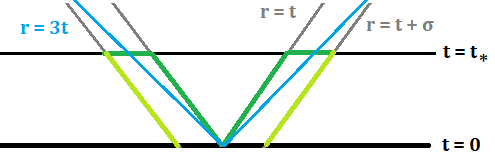
\includegraphics{graphics/exterior}
		\caption{We first choose, via flux decay, a time $t = t_*$ below which the flux is small, and then, via monotone convergence, $\sigma \ll 1$ such that the local energy in the annulus $B_{t_* + \sigma} \setminus B_{t_*}$ at time $t = t_*$ is small. The flux on the exterior cone has the correct sign, so we conclude from the energy-flux identity that the local energy in the annulus is small as $t \downarrow 0$. }
	\end{center}
\end{figure}

\begin{corollary}[Exterior energy decay]\label{cor:exterior}
	Let $\phi \in C^0_{t} \dot H^1_x \cap \dot C^1_{t} L^2_x ((0, 1] \times \R^d)$ be a finite energy local solution to \eqref{NLW}, then
		\[
			\lim_{\sigma \to 0} \limsup_{t \downarrow 0} \cE_{B_{t + \sigma} \setminus B_{t}} [\phi[t]] = 0.
		\]
	In particular, 
		\[
			\limsup_{t \downarrow 0} \cE_{B_{3t} \setminus B_{t}} [\phi[t]] = 0.
		\]	
\end{corollary}

\begin{proof}
	It is clear that for each $\sigma > 0$, we have $B_{3t} \setminus B_t \subseteq B_{t + \sigma} \setminus B_t$ for $t \ll \sigma$, which shows the latter decay statement is implied by the former. To prove the former, let $\epsilon > 0$, we choose from flux decay a time $t_* \ll 1$ such that
		\[
			\cF_{\partial C_{(0, t_*]}} [\phi] \ll \epsilon. 
		\]
	Then, considering the solution on the time slice $t = t_*$, it follows from monotone convergence that there exists $\sigma \ll 1$ such that 
		\[
			\cE_{B_{t_* + \sigma} \setminus B_{t_*}} [\phi[t_*]] \ll \epsilon.
		\]	
	It follows then from the energy-flux identity that, for $t \ll t_*$, 
		\begin{align*}
			 \cE_{B_{t + \sigma} \setminus B_{t}} [\phi[t]] 
			 	&= \cE_{B_{t + \sigma}} [\phi[t]] - \cE_{B_{t}} [\phi[t]] \\
			 	&= \left(\cE_{B_{t_* + \sigma}} [\phi[t_*]] - \cF_{- \sigma + \partial C_{[t, t_*]}} [\phi] \right) - \left( \cE_{B_{t_*}} [\phi[t_*]] - \cF_{\partial C_{[t, t_*]}} [\phi] \right).
		\end{align*}
	Since the flux is non-negative, we can throw away the first flux term, while by our choice of $t_* \ll 1$ and $\sigma \ll 1$ the exterior energy and flux at time $t = t_*$ is small,
		\[
			 \cE_{B_{t + \sigma} \setminus B_{t}} [\phi[t]] \leq  \cE_{B_{t_* + \sigma} \setminus B_{t_*}} [\phi[t_*]] + \cF_{\partial C_{(0, t_*]}} [\phi] \ll \epsilon.  
		\]
	This proves the result.
\end{proof}



\subsection{Monotonicity formula}

We derive a monotonicity formula for the non-linear wave equation arising from the scaling symmetry. The infinitesimal generator of this symmetry is given by $\Lambda = \partial_\rho + \tfrac1\rho$, so, after translating in time $t \mapsto t + \epsilon$ to handle the degeneracy at the light cone, we define 
	\begin{align*}
		X_\epsilon
			&= \frac{1}{\rho_\epsilon} ((t + \epsilon) \partial_t + r \partial_r), \\
		w_\epsilon
			&= \frac{d - 2}{2 \rho_\epsilon},	
	\end{align*}
where $\rho_\epsilon := \sqrt{(t + \epsilon)^2 - r^2}$. Observe that $X_0 = \tfrac1\rho S = \partial_\rho$, where $S$ is the scaling vector field. 
\begin{lemma}[Local monotonicity formula]
	Let $\phi$ be a smooth solution to \eqref{NLW} on an open subset $\cO \subseteq C_{(0, \infty)}$ of the forward light cone. Then the $1$-current defined in null coordinates by 
		\begin{align*}
			{^{(X_\epsilon)}} P_L [\phi]
				&= \frac12 \left( \frac{v_\epsilon}{u_\epsilon} \right)^{1/2} \left| r^{-\frac{d - 2}{2}} L \left( r^{\frac{d - 2}{2}} \phi \right)\right|^2 + \frac12 \left( \frac{u_\epsilon}{v_\epsilon} \right)^\frac12 \left( |\slashed \nabla \phi|^2 + \frac{(d - 2)^2}{4} \frac1{r^2} |\phi|^2 + \frac{d - 2}{d} |\phi|^{\frac{2d}{d - 2}} \right),\\
			{^{(X_\epsilon)}} P_{\underline L} [\phi]
				&= \frac12 \left( \frac{u_\epsilon}{v_\epsilon} \right)^{1/2} \left| r^{-\frac{d - 2}{2}} \underline L \left( r^{\frac{d - 2}{2}} \phi \right)\right|^2 + \frac12 \left( \frac{v_\epsilon}{u_\epsilon} \right)^\frac12 \left(  |\slashed \nabla \phi|^2 + \frac{(d - 2)^2}{4} \frac1{r^2} |\phi|^2 + \frac{d - 2}{d} |\phi|^{\frac{2d}{d - 2}}  \right),
		\end{align*}	
	setting the other components to zero, obeys the divergence identity
		\[
			\partial^\mu \left( {^{(X_\epsilon)}} P_\mu [\phi] \right) = \frac{1}{\rho_\epsilon} \left| \left( \partial_{\rho_\epsilon} + \frac1{\rho_\epsilon} \right)\phi \right|^2.
		\]	
\end{lemma}

\begin{proof}
	See Appendix \ref{app:A}
\end{proof}

Suppose the flux $\cF_{\partial C_{[t_0, t_1]}}[\phi]$ through the null boundary vanishes, then it follows that $\phi$ must also vanish along the null boundary. This kills the null boundary terms when we integrate the local monotonicity formula over the cone $C_{[t_0, t_1]}$ and apply the divergence theorem, thereby furnishing the identity
	\[
			\cM_{S_{t_1}} [\phi] + \iint_{C_{[t_0, t_1]}} \frac1\rho \left| \left( \partial_\rho + \frac1\rho \right) \phi\right|^2 \, dt dx = \cM_{S_{t_0}} [\phi],
	\]
for the weighted energy
	\begin{align*}
		\cM^\epsilon_{S_t} [\phi] 
			&:= \int_{S_t} {^{(X_\epsilon)}}P_T [\phi] \, dx \\
			&= \frac12 \int_{S_t} \left( \frac{v_\epsilon}{u_\epsilon} \right)^{1/2} \left| r^{-\frac{d - 2}{2}} \underline L \left( r^{\frac{d - 2}{2}} \phi \right)\right|^2 + \left( \frac{u_\epsilon}{v_\epsilon} \right)^{1/2} \left| r^{-\frac{d - 2}{2}} L \left( r^{\frac{d - 2}{2}} \phi \right)\right|^2 \\
			&\qquad + \left( \left( \frac{v_\epsilon}{u_\epsilon}\right)^\frac12  + \left( \frac{u_\epsilon}{v_\epsilon} \right)^\frac12 \right) \left(  |\slashed \nabla \phi|^2 + \frac{(d - 2)^2}{4} \frac1{r^2} |\phi|^2 + \frac{d - 2}{d} |\phi|^{\frac{2d}{d - 2}}  \right)	dx.
	\end{align*}
Since the second term is non-negative, this implies monotonocity of $\cM_{S_{t}}[\phi]$. In particular, the second term vanishes as $t_0, t_1 \to 0$, implying that rescalings of $\phi$ are asymptotically self-similar. On the other hand, the weights $(\tfrac{v}{u})^{1/2}$ blow-up at the null boundary, so there cannot be null concentration of energy. In the case where the flux does not vanish, we can still prove an "almost" monotonicity formula, leveraging the flux decay and a local Hardy's inequality to control the $\tfrac{|\phi|^2}{r^2}$ terms in the weighted energy. Before stating the almost monotonicity formula, we state and prove this Hardy decay. Define 
	\[
		\cG_{\partial S_t} [\phi]
			:= \frac1t \int_{\partial S_t} |\phi|^2.
	\]
This is well-defined for finite-energy solutions by the Sobolev trace theorem; in fact, $\phi \in H^{1/2}(\partial S_t)$.  

\begin{proposition}[Local Hardy's inequality]
	Let $\phi \in C^0_{t, \loc} \dot H^1_x \cap \dot C^1_{t, \loc} L^2_x (I \times \R^d)$, then
		\[
			\cG_{\partial S_{t_0}} [\phi] + \int_{t_0}^{t_1} \cG_{\partial S_t} [\phi] \frac{dt}{t} \leq \cG_{\partial S_{t_1}} [\phi] + \cF_{\partial C_{[t_0, t_1]}} [\phi].
		\]
	and 
		\[
			\cG_{\partial S_t} [\phi] \leq \cE_{\{t\} \times \R^d \setminus S_t} [\phi].
		\]		
\end{proposition}

\begin{proof}
	Standard proof of Hardy's inequality adapted to the null cone. 
\end{proof}

\begin{corollary}[Decay of Hardy term]
	Let $\phi \in C^0_{t, \loc} \dot H^1_x \cap \dot C^1_{t, \loc} L^2_x (I \times \R^d)$ be a strong solution to \eqref{NLW}, then $\cG_{\partial S_t} [\phi]$ vanishes as $t \to 0$ and $t \to \infty$,
		\begin{align*}
			\lim_{t \downarrow 0}\cG_{\partial S_t} [\phi]
				&= 0, \\
			\lim_{t \uparrow \infty}\cG_{\partial S_t} [\phi]
				&= 0.	
		\end{align*}	
\end{corollary}

\begin{proof}
	The local Hardy's inequality and finite energy implies that $\int \tfrac1t \cG_{\partial S_t} [\phi] < \infty$. We claim that if $\cG_{\partial S_t} [\phi]$ does not decay as $t\downarrow 0$ or $t\uparrow \infty$, then we can extract a uniform lower bound for either $t \ll 1$ or $t \gg 1$ respectively, a contradiction since $\int \tfrac1t$ diverges logarithmically. Suppose the $t \downarrow 0$ case fails; the case $t \uparrow \infty$ is similar, then local Hardy implies
		\[
			0 < \limsup_{t \downarrow 0} \cG_{\partial S_t} [\phi] \leq \cG_{S_t} [\phi] + \cF_{\partial C_{[0, t]}}.
		\]
	By flux decay, the flux term can be absorbed into the left-hand side for $t \ll 1$, proving the claim. 
\end{proof}

\begin{theorem}[Almost monotonicity formula I]\label{thm:monotone1}
	Let $\phi$ be a strong solution to \eqref{NLW} on $[\epsilon, 1] \times \R^d$ with negligible flux through the null boundary, finite energy and negligible Hardy term at $t = 1$, 
	\begin{align*}
		\cE_{S_1} [\phi]
			&\leq \cE, \\
		\cF_{\partial C_{[\epsilon, 1]}} [\phi]
			&\leq \epsilon^{1/2} \cE, \\
		\cG_{\partial S_1}[\phi]
			&\leq \epsilon^{1/2}\cE.
	\end{align*} 
	Then
		\[
			\cM_{S_{1}}^\epsilon [\phi] + \iint_{C_{[\epsilon, 1]}} \frac1{\rho_\epsilon} \left| \left( \partial_{\rho_\epsilon} + \frac1{\rho_\epsilon} \right) \phi\right|^2 \, dt dx \lesssim \cE.
		\]	
\end{theorem}

\begin{proof}
	Approximating a strong solution in the energy topology, it suffices to consider smooth solutions. We integrate the local monotonicity formula over the cone $C_{[\epsilon, 1]}$ and apply the divergence theorem, 
		\begin{align*}
			\cM_{S_{1}}^\epsilon [\phi] + \iint_{C_{[\epsilon, 1]}} \frac1{\rho_\epsilon} \left| \left( \partial_{\rho_\epsilon} + \frac1{\rho_\epsilon} \right) \phi\right|^2 \, dt dx 
				&=\cM_{S_{\epsilon}}^\epsilon [\phi] + \frac12 \int_{\partial C_{[\epsilon, 1]}} {^{(X_\epsilon)}}P_L [\phi] \, dS.
		\end{align*}
	We claim that the right-hand side is controlled by $\cE$.
	
	To control the weighted energy $\cM^\epsilon_{S_\epsilon} [\phi]$ on the time slice $S_\epsilon$, we first note that the weights can be treated as constants $|\tfrac{v_\epsilon}{u_\epsilon}| \sim |\tfrac{u_\epsilon}{v_\epsilon}| \sim 1$. It follows that we can estimate the integrand of the weighted energy $\cM^\epsilon_{S_\epsilon} [\phi]$ by the integrand of the local energy $\cE_{S_\epsilon} [\phi]$ and the Hardy term $\tfrac{|\phi|^2}{r^2}$, e.g.
		\begin{align*}
			\left(\frac{v_\epsilon}{u_\epsilon} \right)^{1/2} \left| r^{-\frac{d - 2}{2}} \underline L \left( r^{\frac{d - 2}{2}} \phi \right)\right|^2 + \left( \frac{u_\epsilon}{v_\epsilon} \right)^{1/2} \left| r^{-\frac{d - 2}{2}} L \left( r^{\frac{d - 2}{2}} \phi \right)\right|^2 
				&\lesssim  \left| r^{-\frac{d - 2}{2}} \underline L \left( r^{\frac{d - 2}{2}} \phi \right)\right|^2 + \left| r^{-\frac{d - 2}{2}} L \left( r^{\frac{d - 2}{2}} \phi \right)\right|^2 \\
				&\lesssim |\partial_t \phi|^2 + |\partial_r \phi|^2 + \frac{|\phi|^2}{r^2},
		\end{align*}
	and similarly for the other terms, so in total
		\[
			\cM^\epsilon_{S_\epsilon} [\phi] \lesssim \cE_{S_\epsilon} [\phi] + \int_{S_\epsilon} \frac{|\phi|^2}{r^2} \, dx \lesssim \cE
		\]	
	by finite energy, which controls $\cE_{S_\epsilon} [\phi]$, and negligible flux and Hardy term, which controls the right-hand side of the local Hardy's inequality. 

	To control the weighted flux term on the null boundary $\partial C_{[\epsilon, 1]}$, we observe that the weights are bounded above $|\tfrac{u_\epsilon}{v_\epsilon}| \leq 1$ and $|\tfrac{v_\epsilon}{u_\epsilon}| \lesssim \tfrac1\epsilon$ in this region. It follows that we can estimate the integrand of the weighted flux by the integrand of the usual flux $\cF_{[\epsilon, 1]}[\phi]$ and the Hardy term $\tfrac{|\phi|^2}{r^2}$, e.g.
		\begin{align*}
			^{(X_\epsilon)} P_L [\phi] \lesssim \epsilon^{-1/2} \left( |L\phi|^2 + \frac{|\phi|^2}{r^2} \right) + {^{(T)}} J_L [\phi],
		\end{align*}
	on the null boundary $\partial C_{[\epsilon, 1]}$, so integrating and applying the negligible flux and Hardy assumptions, 
		\[
			\int_{\partial C_{[\epsilon, 1]}} {^{(X_\epsilon)}} P_L [\phi] \, dS \lesssim \cE.
		\]	
	This completes the proof. 	
\end{proof}


\begin{corollary}[Almost monotonicity formula II]\label{thm:monotone2}
	Let $\phi$ be a strong solution to \eqref{NLW} on $[\epsilon, 1] \times \R^d$ satisfying the hypotheses of Theorem \ref{thm:monotone1}. Then
		\[
			\cM_{S^{\delta_1}_1} [\phi] \lesssim \cM_{S^{\delta_0}_{t_0}} [\phi] + \left( \left( \frac{\delta_1}{t_0}\right)^{1/2} + \frac{1}{|\log (\delta_1/\delta_0)|} \right) \cE
		\]	
	whenever $2\epsilon \leq \delta_0 \leq \delta_1 \leq t_0$. 	
\end{corollary}

\begin{proof}
	For any $\delta \in [\delta_0, \delta_1]$, we have that $S^{\delta_1}_1 \subseteq S^\delta_1$ and $S^{\delta_0}_{t_0} \subseteq S^{\delta}_{t_0}$. Thus, integrating the local monotonicity formula over the translated cone $C^\delta_{[t_0, 1]}$ and applying the divergence theorem, we see that it suffices to control the flux term 
		\[
			\int_{\partial C^\delta_{[t_0, 1]}} {^{(X)}} P_L [\phi] \, dS \lesssim  \left( \left( \frac{\delta_1}{t_0}\right)^{1/2} + \frac{1}{|\log (\delta_1/\delta_0)|} \right) \cE
		\]
	for appropriately chosen $\delta$. We control the term with $\tfrac{u}{v}$ weight by localised Hardy and local conservation of energy, 
		\begin{align*}
			\int_{\partial C^\delta_{[t_0, 1]}} &\left( \frac{u}{v} \right)^\frac12 \left( |\slashed \nabla \phi|^2 + \frac{(d - 2)^2}{4} \frac1{r^2} |\phi|^2 + \frac{d - 2}{d} |\phi|^{\frac{2d}{d - 2}} \right) dS\\
				 &\lesssim \left( \frac{\delta_1}{t_0} \right)^{1/2} \left( \cF_{\partial C^\delta_{[t_0, 1]}} [\phi] + \cE_{S_1 \setminus S_1^\delta} [\phi] + \cG_{S_1} [\phi]  \right) \lesssim  \left( \frac{\delta_1}{t_0} \right)^{1/2} \cE. 
		\end{align*}
	To treat the term with $\tfrac{v}{u}$ weight, we compute
		\[
			r^{-\frac{d - 2}{2}} L\left( r^{\frac{d- 2}{2}} \phi \right) = \left( L + \frac{d - 2}{2}\frac1r \right) \phi.
		\]	
	Finite energy plus pigeonhole principle. 	
\end{proof}